%  !TeX  root  =  user_guide.tex

\section{Модуль Преобразователь Dxf2Shp}

% когда переработка раздела будет завершена,
% раскоментируйте следующую строку:
%\updatedisclaimer

Модуль Преобразователь dxf2shape может быть использован для преобразования
векторных данных из формата DXF в формат shape-файлов. Перед его
использованием должны быть определены следующие параметры:

\begin{itemize}
\item \textbf{Входной DXF-файл}: Введите путь до файла в формате DXF,
который необходимо преобразовать
\item \textbf{Выходной Shp-файл}: Введите любое желаемое имя файла для
создаваемого shape-файла
\item \textbf{Тип выходного файла}: Определите тип геометрии данных
выходного shape-файла. В настоящее время поддерживаются такие типы как
полилиния, полигон и точка.
\item \textbf{Экспорт текстовых меток}: При выборе данного пункта
дополнительно будет создан shape-файл слоя точек, ассоциированный с
таблицей dbf, которая содержит информацию о полях <<TEXT>>, найденных в
файле dxf и соответствующие текстовые строки.
\end{itemize}

\begin{figure}[ht]
   \centering
   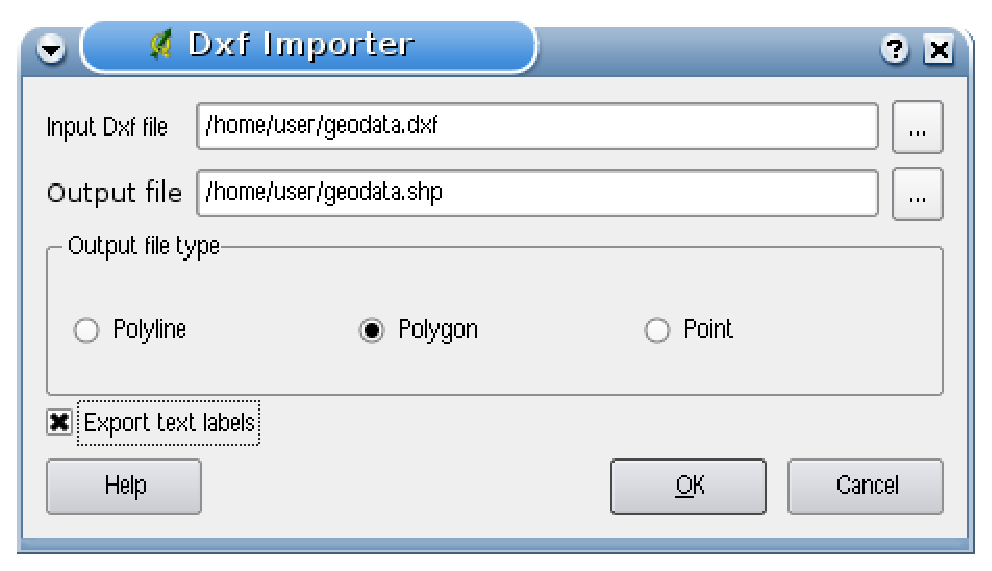
\includegraphics[clip=true, width=12cm]{dxf2shape_dialog}
   \caption{Модуль Преобразователь Dxf2Shape \nixcaption}\label{fig:dxf2shape_dialog}
\end{figure}

\minisec{Использование модуля}

\begin{enumerate}
  \item Запустите QGIS, загрузите модуль Dxf2Shape в Менеджере модулей
  (см. Раздел~\ref{sec:load_core_plugin}) и нажмите кнопку
  \toolbtntwo{dxf2shp_converter}{Dxf2Shape Converter} расположенную на
  панели инструментов QGIS. Диалоговое окно модуль Dxf2Shape показано на
  Рисунке~\ref{fig:dxf2shape_dialog}.
  \item Введите имя входного DXF файла, укажите имя выходного shape-файла
  и его тип.
  \item Выберите пункт \checkbox{Экспорт текстовых меток} если вам
  требуется создать дополнительный слой содержащий надписи.
  \item Нажмите кнопку \button{Ok}.
\end{enumerate}

\FloatBarrier
